% Collapsing Decision Boundaries -- TU Dortmund-style 4:3 Beamer deck
% Compile with: latexmk -pdf DDM_Final_presentation.tex
% Presenter handoffs are marked in comments: 1--4, 5--9, 10--13, and 14--18.
\documentclass[aspectratio=43,10pt]{beamer}

\usepackage[utf8]{inputenc}
\usepackage[T1]{fontenc}
\usepackage[scaled=0.92]{helvet}
\renewcommand{\familydefault}{\sfdefault}
\usepackage{amsmath}
\usepackage{array}
\usepackage{booktabs}
\usepackage{graphicx}
\usepackage{ragged2e}
\usepackage{tabularx}

\graphicspath{{presentation_assets/}}

\definecolor{TUGreen}{HTML}{78BE20}
\definecolor{TULightGreen}{HTML}{B7D98A}
\definecolor{TUDark}{HTML}{203A3E}
\definecolor{TUText}{HTML}{30383B}
\definecolor{TUMuted}{HTML}{687377}
\definecolor{TUBlue}{HTML}{355C8C}
\definecolor{TUWarn}{HTML}{A9503A}

\setbeamercolor{normal text}{fg=TUText,bg=white}
\setbeamercolor{frametitle}{fg=white,bg=TUDark}
\setbeamercolor{structure}{fg=TUText}
\setbeamercolor{itemize item}{fg=TUText}
\setbeamercolor{itemize subitem}{fg=TUText}
\setbeamerfont{title}{size=\fontsize{24}{28},series=\mdseries}
\setbeamerfont{author}{size=\fontsize{13}{16}}
\setbeamerfont{institute}{size=\fontsize{10}{12}}
\setbeamerfont{frametitle}{size=\fontsize{17}{20},series=\mdseries}
\setbeamerfont{normal text}{size=\fontsize{13}{16}}

\setbeamertemplate{navigation symbols}{}
\setbeamertemplate{itemize item}{\color{TUGreen}\large\textbullet}
\setbeamertemplate{itemize subitem}{\color{TUGreen}\normalsize\textbullet}
\setlength{\leftmargini}{1.25em}
\setlength{\leftmarginii}{1.25em}
\setbeamersize{text margin left=0.70cm,text margin right=0.70cm}

% Header, underline, and footer follow the supplied TU Dortmund brief.
\setbeamertemplate{frametitle}{%
  \nointerlineskip
  \begin{beamercolorbox}[wd=\paperwidth,ht=0.68cm,dp=0.18cm,leftskip=0.55cm]{frametitle}
    \usebeamerfont{frametitle}\insertframetitle
  \end{beamercolorbox}%
  \nointerlineskip
  \hbox{\color{TUGreen}\rule{1.20cm}{1.1pt}\color{TULightGreen}\rule{\dimexpr\paperwidth-1.20cm\relax}{0.45pt}}%
}

\setbeamertemplate{footline}{%
  \ifnum\insertframenumber=1\relax\else
    \hbox to \paperwidth{\hfill\color{TUMuted}\fontsize{7.5}{9}\selectfont\insertframenumber\hspace{0.45cm}}%
  \fi
}

\newcommand{\slidecaption}[1]{%
  {\color{TUMuted}\fontsize{8.5}{10.5}\selectfont #1\par}%
}
\newcommand{\greenheading}[1]{%
  {\color{TUGreen}\fontsize{12}{14}\selectfont\bfseries #1\par}%
}
\newcommand{\metric}[2]{%
  {\color{TUGreen}\fontsize{20}{22}\selectfont\bfseries #1}\\[-0.06cm]
  {\fontsize{9.5}{11.5}\selectfont #2}%
}

\title{Collapsing Decision Boundaries}
\author{Anirudh Parameswaran\\Gautam Dilip Hariharan}
\institute{TU Dortmund University}
\date{}

\begin{document}

% -----------------------------------------------------------------------------
% Presenter 1 -- Motivation and question
% -----------------------------------------------------------------------------
\begin{frame}[plain]
  \vspace{0.20cm}
  \hfill
\includegraphics[width=4.15cm]{tu_dortmund_logo.png}

  \vspace{1.05cm}
  {\usebeamerfont{title}\color{TUText}\inserttitle\par}
  \vspace{0.45cm}
  {\color{TUGreen}\rule{\textwidth}{0.7pt}}

  \vspace{0.55cm}
  {\usebeamerfont{author}\color{TUText}\insertauthor\par}
  \vspace{0.25cm}
  {\usebeamerfont{institute}\color{TUText}\insertinstitute\par}
\end{frame}

\begin{frame}{Introduction}
  \vspace{0.20cm}
  \greenheading{Fast decisions are everywhere}
  \vspace{0.14cm}
  \begin{itemize}
    \item Was that a green or red light?
    \item Do I press left or right?
    \item In two-choice experiments, we record both the response and the response time.
  \end{itemize}

  \vspace{0.30cm}
  \greenheading{The speed--accuracy question}
  \begin{itemize}
    \item How does a person change their decision process when time pressure increases?
    \item A drift diffusion model represents a decision as evidence accumulating until a choice is made.
  \end{itemize}
\end{frame}

\begin{frame}{Why collapsing boundaries?}
  \vspace{0.14cm}
  \greenheading{Evidence from deadline experiments}
  \begin{itemize}
    \item Fixed boundaries can describe instructions to respond quickly.
    \item Explicit deadlines create increasing urgency; collapsing boundaries can describe this pressure better.
    \item We investigate a curved, exponential collapse rather than a constant linear decline.
  \end{itemize}

  \vspace{0.38cm}
  \begin{center}
    \begin{tabular}{c@{\hspace{1.0cm}}c}
      \textbf{Fixed threshold} & \textbf{Collapsing threshold} \\
      $a(t)=a$ & $a(t)\ \downarrow\ \text{as time passes}$
    \end{tabular}
  \end{center}

  \vspace{0.38cm}
  {\color{TUMuted}\fontsize{10}{12}\selectfont
  Motivation: under a deadline, the amount of evidence required for a decision may decrease over time (Katsimpokis et al., 2020).}
\end{frame}

\begin{frame}{Research question}
  \vspace{0.20cm}
  \greenheading{What remains unexplored?}
  \begin{itemize}
    \item Non-linear boundary collapse, including exponential and sigmoid functions.
    \item Urgency mechanisms that change the decision process as time passes.
  \end{itemize}

  \vspace{0.45cm}
  \greenheading{Our question}
  {\fontsize{17}{21}\selectfont
  Can an exponentially collapsing boundary explain speed and accuracy across deadline and cue conditions?\par}

  \vspace{0.38cm}
  {\color{TUMuted}\fontsize{10.5}{13}\selectfont
  We answer this with simulation-based inference, recovery diagnostics, and posterior predictive checks.}
\end{frame}

% -----------------------------------------------------------------------------
% Presenter 2 -- Model, inference, and prior predictive validation
% -----------------------------------------------------------------------------
\begin{frame}{The evidence accumulation model}
  \vspace{0.08cm}
  \begin{columns}[T,onlytextwidth]
    \begin{column}{0.47\textwidth}
      \centering
      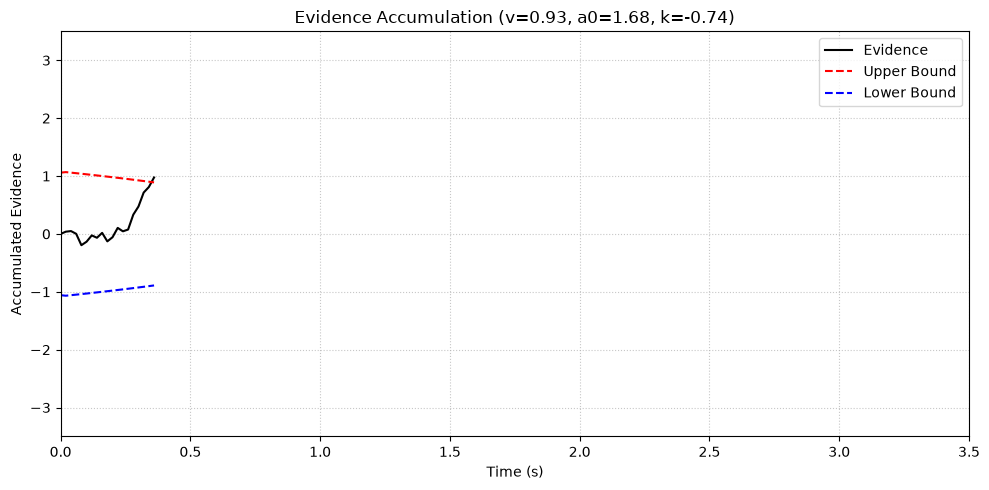
\includegraphics[width=\linewidth]{ddm_trajectory.png}
      \slidecaption{Figure: a simulated evidence path reaching a collapsing bound.}
    \end{column}
    \begin{column}{0.49\textwidth}
      \greenheading{Drift diffusion model}
      \vspace{0.06cm}
      \begin{equation*}
        \mathrm{d}x = \nu\,\mathrm{d}t + \sqrt{\mathrm{d}t}\,\varepsilon
      \end{equation*}
      \begin{itemize}
        \item $\nu$: average evidence drift
        \item a decision occurs when evidence hits an upper or lower boundary
        \item the simulator returns a response time and a binary response
      \end{itemize}
      \vspace{0.12cm}
      {\color{TUMuted}\fontsize{9.5}{11.5}\selectfont
      The model has no non-decision-time or trial-to-trial variability component.}
    \end{column}
  \end{columns}
\end{frame}

\begin{frame}{Exponential boundary collapse}
  \vspace{0.17cm}
  \greenheading{Why use a non-linear collapse?}
  \begin{itemize}
    \item A linear boundary assumes constant pressure to decide.
    \item A curved boundary permits slower early decline and a sharper late drop near the deadline.
  \end{itemize}

  \vspace{0.35cm}
  \begin{center}
    {\fontsize{21}{25}\selectfont
      $a(t)=a_0\left[1-\exp\left(k(T-t)\right)\right]$}
  \end{center}

  \vspace{0.32cm}
  \begin{tabularx}{\textwidth}{>{\raggedright\arraybackslash}X >{\raggedright\arraybackslash}X >{\raggedright\arraybackslash}X}
    $a_0$: boundary scale & $k<0$: collapse curvature & $T=1.35$ s: decision horizon
  \end{tabularx}

  \vspace{0.30cm}
  {\color{TUMuted}\fontsize{9.8}{12}\selectfont
  More negative $k$ keeps the boundary higher early and makes its decline steeper near $T$.}
\end{frame}

\begin{frame}{BayesFlow: simulated data}
  \vspace{0.08cm}
  \greenheading{A simulator supplies labeled examples}
  \begin{itemize}
    \item One simulated data set contains 200 response times and binary responses.
    \item The simulator also knows the generating values of $\nu$, $k$, and $a_0$.
    \item 5,000 simulated data sets form the offline training set; 100 are held out for validation.
    \item This creates the learning task: infer the three latent parameters from a set of trials.
  \end{itemize}
\end{frame}

\begin{frame}{BayesFlow: inference and training}
  \vspace{0.08cm}
  \greenheading{From trial set to posterior distribution}
  \begin{itemize}
    \item A DeepSet network summarizes the unordered set of RT and binary-response trials.
    \item A flow-matching inference network (depth 8) maps this summary to posterior samples of $\nu$, $k$, and $a_0$.
    \item The adapter constrains $k<0$ and $a_0>0$, standardizes variables, and concatenates parameters for inference.
    \item Training uses 150 epochs, batch size 100, and an initial learning rate of $10^{-3}$.
  \end{itemize}

  \vspace{0.38cm}
  {\color{TUMuted}\fontsize{10}{12}\selectfont
  After training, the same amortized network samples a posterior for each empirical condition without retraining.}
\end{frame}

\begin{frame}{Prior predictive check}
  \vspace{0.02cm}
  \begin{columns}[T,onlytextwidth]
    \begin{column}{0.47\textwidth}
      \greenheading{Finalized prior}
      {\fontsize{8.9}{11}\selectfont
      \begin{align*}
        \nu &\sim \mathcal{N}(1.2,1.0), \\
        k &= -0.6-0.4\,\Gamma(2,0.5), \\
        a_0 &= 1.6+0.15\,\Gamma(2,0.5).
      \end{align*}}
      \vspace{-0.16cm}
      \greenheading{Empirical vs. prior summary}
      \vspace{0.10cm}
      {\fontsize{7.9}{9.8}\selectfont
      \begin{tabularx}{\linewidth}{>{\raggedright\arraybackslash}X r r}
        \toprule
        & \textbf{Prior} & \textbf{Empirical} \\
        \midrule
        Accuracy & 0.804 & 0.810 \\
        Mean RT (s) & 0.598 & 0.604 \\
        SD RT (s) & 0.293 & 0.431 \\
        Median RT (s) & 0.560 & 0.527 \\
        10\% quantile & 0.240 & 0.293 \\
        90\% quantile & 1.040 & 0.926 \\
        \bottomrule
      \end{tabularx}}

      \vspace{0.16cm}
      {\color{TUMuted}\fontsize{8.6}{10.5}\selectfont
      We experimented with different priors and retained this one because it produced plausible central RT and response behavior before training.}
    \end{column}
    \begin{column}{0.50\textwidth}
      \centering
      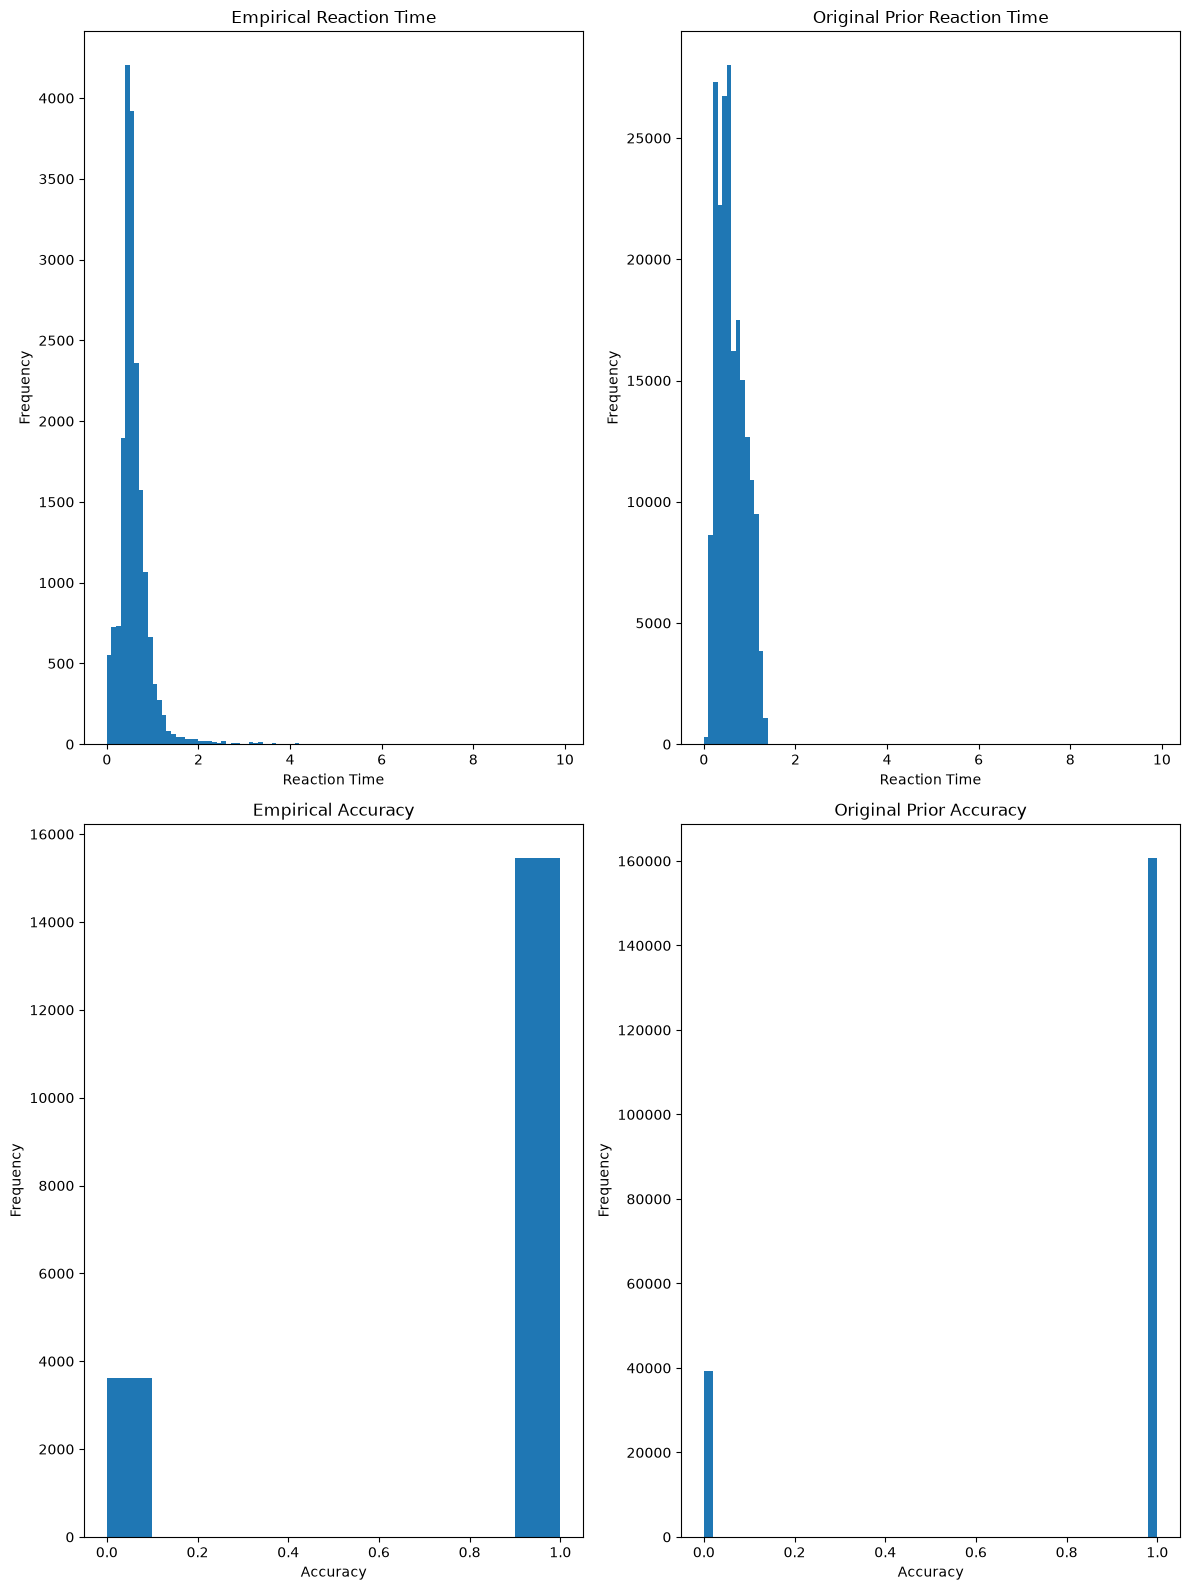
\includegraphics[width=\linewidth,height=6.35cm,keepaspectratio]{prior_predictive_check.png}
      \slidecaption{Figure: empirical and prior-predictive reaction-time and binary-response distributions.}
    \end{column}
  \end{columns}
\end{frame}

% -----------------------------------------------------------------------------
% Presenter 3 -- Simulation-based validation
% -----------------------------------------------------------------------------
\begin{frame}{Stable training over 150 epochs}
  \vspace{0.15cm}
  \centering
  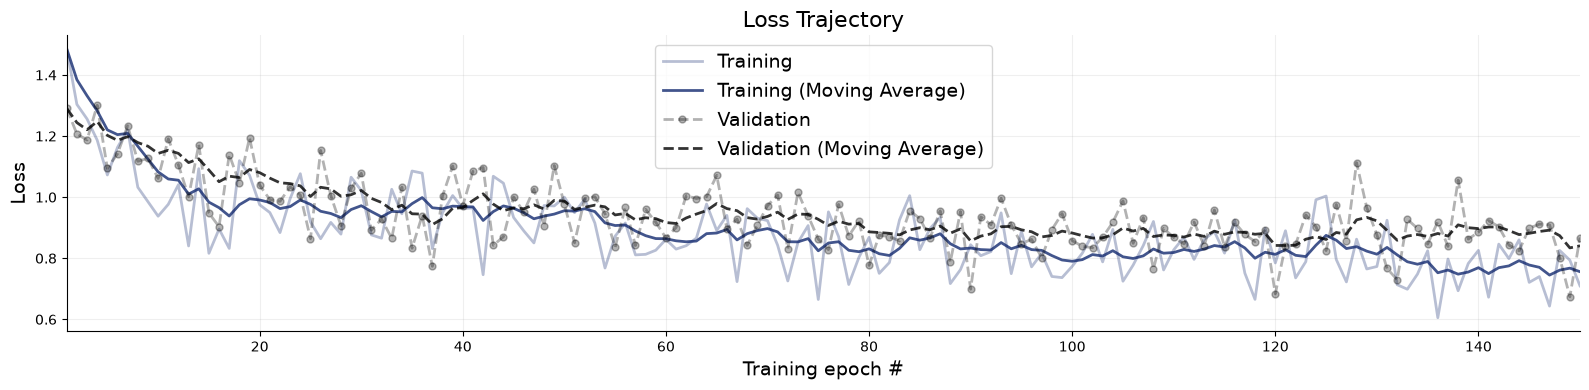
\includegraphics[width=0.97\textwidth]{diagnostic_loss.png}
  \vspace{0.06cm}
  \slidecaption{Figure: training and validation loss trajectories. Both moving averages decrease without obvious divergence.}
\end{frame}

\begin{frame}{Parameter recovery}
  \vspace{0.10cm}
  \centering
  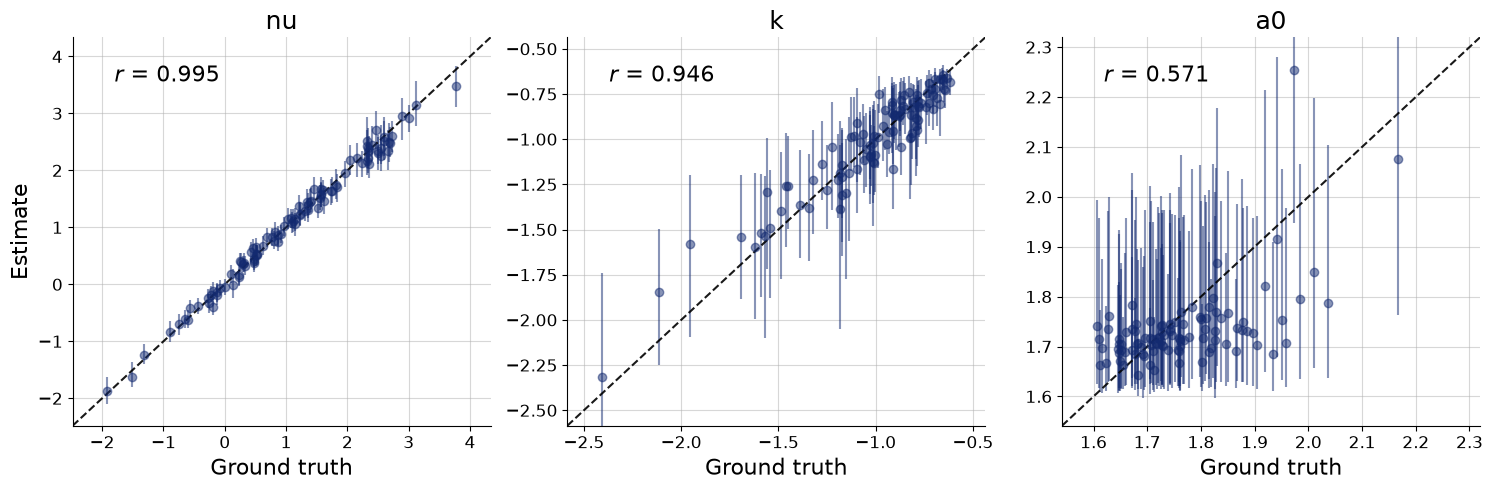
\includegraphics[width=0.98\textwidth]{diagnostic_recovery.png}
  \vspace{0.08cm}
  \begin{columns}[T,onlytextwidth]
    \begin{column}{0.32\textwidth}\centering\metric{$r=0.995$}{drift $\nu$}\end{column}
    \begin{column}{0.32\textwidth}\centering\metric{$r=0.946$}{collapse $k$}\end{column}
    \begin{column}{0.32\textwidth}\centering\metric{$r=0.571$}{scale $a_0$}\end{column}
  \end{columns}
\end{frame}

\begin{frame}{Simulation-based calibration}
  \vspace{0.18cm}
  \centering
  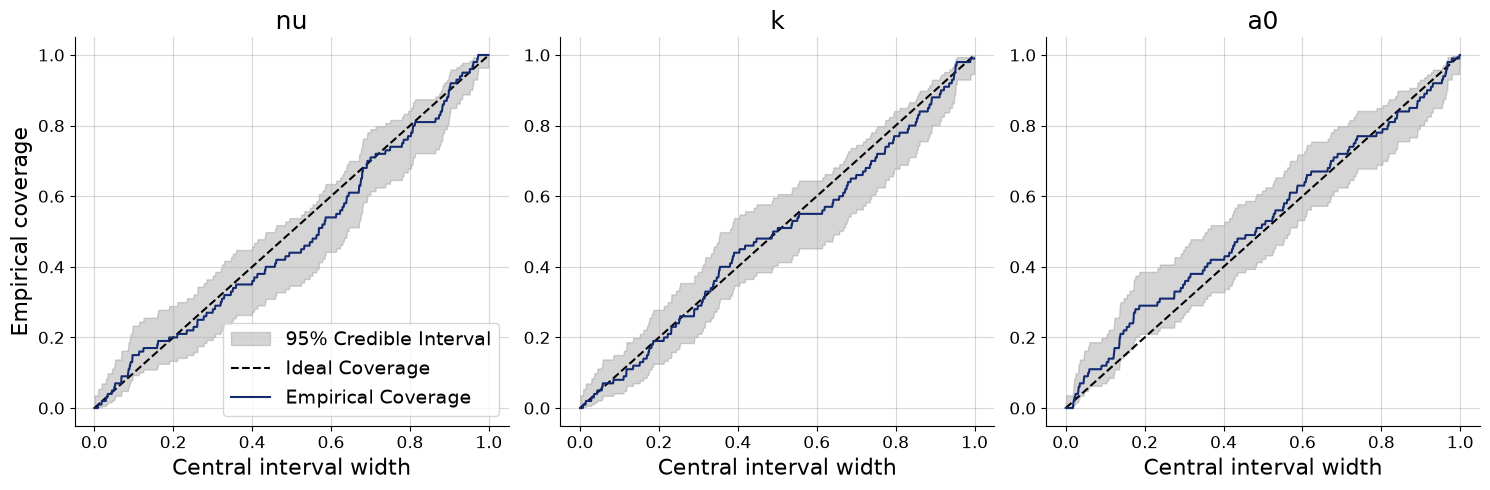
\includegraphics[width=0.97\textwidth]{diagnostic_sbc.png}
  \vspace{0.10cm}
  \slidecaption{Figure: empirical coverage against central interval width. Curves remain within the 95\% reference bands.}
\end{frame}

\begin{frame}{Posterior contraction}
  \vspace{0.18cm}
  \centering
  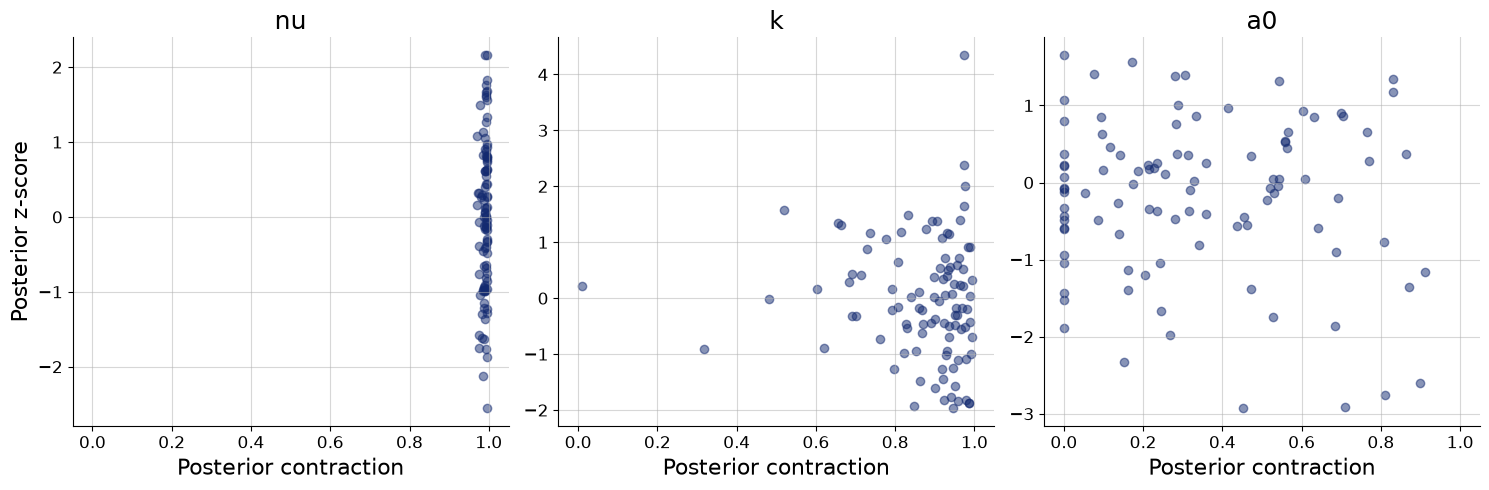
\includegraphics[width=0.97\textwidth]{diagnostic_contraction.png}
  \vspace{0.09cm}
  \slidecaption{Figure: posterior z-score against posterior contraction. Drift is strongly contracted; $a_0$ is much more scattered.}
\end{frame}

% -----------------------------------------------------------------------------
% Presenter 4 -- Empirical data and posterior predictive validation
% -----------------------------------------------------------------------------
\begin{frame}{Testing the experimental data}
  \vspace{0.10cm}
  \greenheading{Four deadline-by-cue conditions}
  \vspace{0.10cm}
  {\fontsize{10.2}{12.5}\selectfont
  \begin{tabularx}{\textwidth}{>{\raggedright\arraybackslash}X r r r}
    \toprule
    \textbf{Condition} & \textbf{Trials} & \textbf{Mean RT (s)} & \textbf{Accuracy} \\
    \midrule
    Deadline -- AC & 4,732 & 0.564 & 0.844 \\
    Deadline -- SP & 4,743 & 0.493 & 0.722 \\
    No deadline -- AC & 4,799 & 0.784 & 0.891 \\
    No deadline -- SP & 4,798 & 0.572 & 0.783 \\
    \bottomrule
  \end{tabularx}}

  \vspace{0.42cm}
  \begin{columns}[T,onlytextwidth]
    \begin{column}{0.46\textwidth}\metric{19,072}{trials in the complete data set}\end{column}
    \begin{column}{0.46\textwidth}\metric{800}{trials per condition for posterior sampling}\end{column}
  \end{columns}

  \vspace{0.28cm}
  {\color{TUMuted}\fontsize{9.8}{12}\selectfont
  AC responses are slower and more accurate than SP responses under both deadline regimes.}
\end{frame}

\begin{frame}{Posterior estimates and PPCs}
  \vspace{0.03cm}
  \begin{columns}[T,onlytextwidth]
    \begin{column}{0.50\textwidth}
      \greenheading{Posterior means}
      {\fontsize{7.7}{9.5}\selectfont
      \begin{tabularx}{\linewidth}{>{\raggedright\arraybackslash}X r r r}
        \toprule
        \textbf{Condition} & $\boldsymbol{\nu}$ & $\boldsymbol{k}$ & $\boldsymbol{a_0}$ \\
        \midrule
        Deadline -- AC & 1.15 & -1.17 & 1.75 \\
        Deadline -- SP & 0.85 & -0.66 & 1.67 \\
        No deadline -- AC & 1.25 & -1.96 & 1.87 \\
        No deadline -- SP & 0.78 & -0.74 & 1.67 \\
        \bottomrule
      \end{tabularx}}
      \vspace{0.20cm}
      {\color{TUMuted}\fontsize{8.5}{10.5}\selectfont
      AC has higher inferred drift than SP in both deadline regimes. Treat $a_0$ differences cautiously.}
    \end{column}
    \begin{column}{0.47\textwidth}
      \greenheading{Average posterior predictive fit}
      {\fontsize{7.7}{9.5}\selectfont
      \begin{tabularx}{\linewidth}{>{\raggedright\arraybackslash}X c c}
        \toprule
        \textbf{Condition} & \textbf{Acc. O/P} & \textbf{RT O/P} \\
        \midrule
        Deadline -- AC & .846 / .884 & .658 / .689 \\
        Deadline -- SP & .790 / .786 & .502 / .518 \\
        No deadline -- AC & .948 / .923 & .918 / .828 \\
        No deadline -- SP & .763 / .771 & .552 / .568 \\
        \bottomrule
      \end{tabularx}}
      \vspace{0.20cm}
      {\color{TUGreen}\fontsize{13}{15}\selectfont\bfseries 4 / 4}\;{\fontsize{8.5}{10.5}\selectfont observed accuracies lie inside the 95\% predictive interval.}
    \end{column}
  \end{columns}

  \vspace{0.26cm}
  {\color{TUMuted}\fontsize{8.8}{10.8}\selectfont
  O/P = observed / posterior-predictive mean. Each check uses 50 replicated data sets with 800 trials each.}
\end{frame}

\begin{frame}{PPCs: deadline trials}
  \vspace{0.01cm}
  \centering
  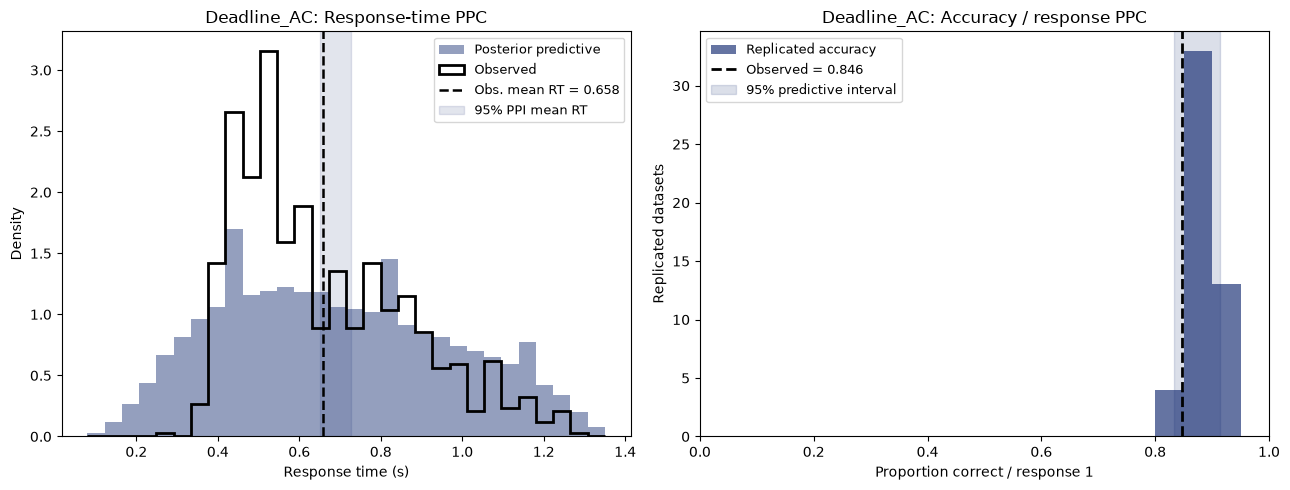
\includegraphics[width=0.82\textwidth]{ppc_deadline_ac.png}
  \vspace{-0.12cm}
  \slidecaption{Deadline--AC: central response-time mass and response proportion are close.}
  \vspace{0.04cm}
  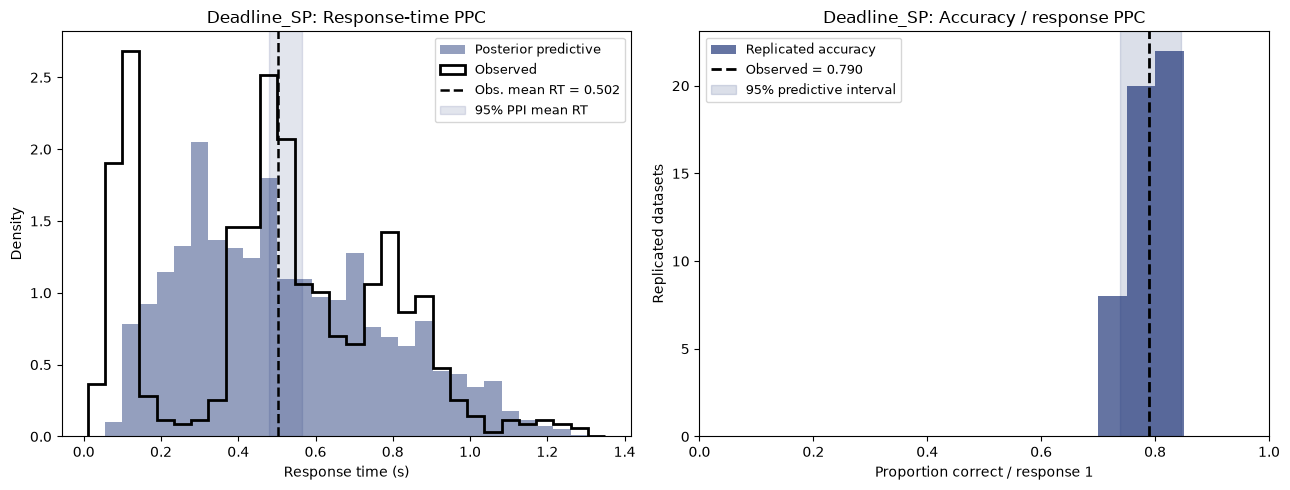
\includegraphics[width=0.82\textwidth]{ppc_deadline_sp.png}
  \vspace{-0.12cm}
  \slidecaption{Deadline--SP: average fit is adequate, while the response-time shape remains simplified.}
\end{frame}

\begin{frame}{PPCs: no-deadline trials}
  \vspace{0.01cm}
  \centering
  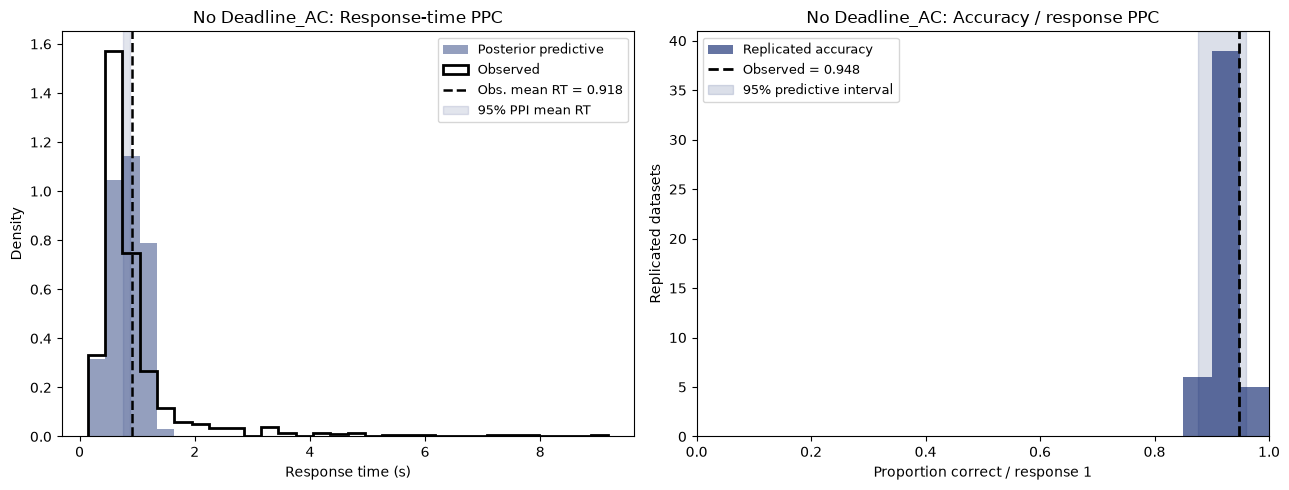
\includegraphics[width=0.82\textwidth]{ppc_no_deadline_ac.png}
  \vspace{-0.12cm}
  \slidecaption{No-deadline--AC: observed accuracy is reproduced, but the long RT tail is absent.}
  \vspace{0.04cm}
  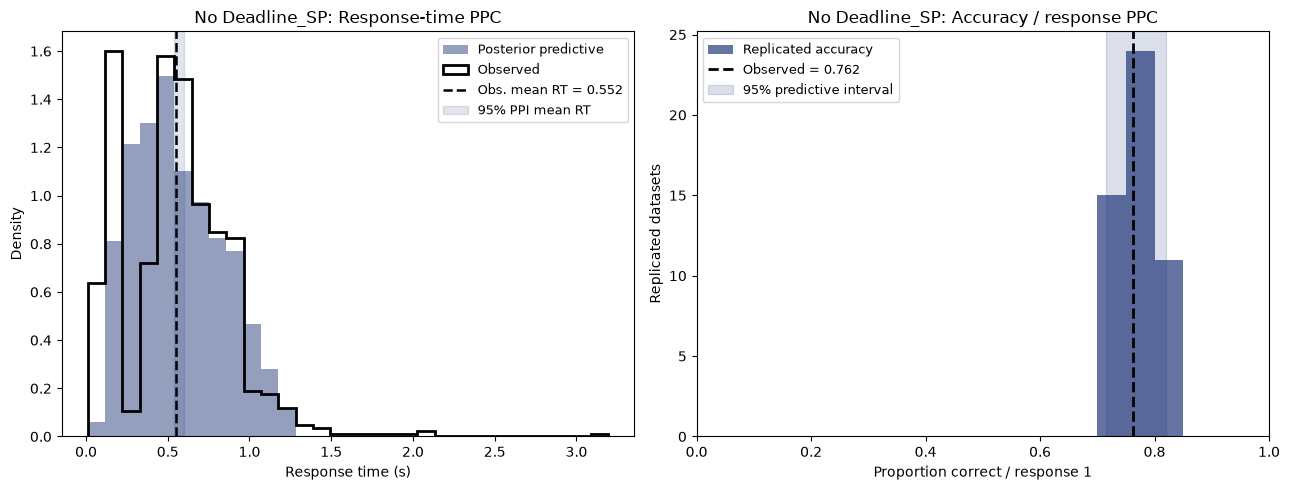
\includegraphics[width=0.82\textwidth]{ppc_no_deadline_sp.png}
  \vspace{-0.12cm}
  \slidecaption{No-deadline--SP: the simulated distribution still terminates at the fixed 1.35 s horizon.}
\end{frame}

\begin{frame}{Conclusion and next steps}
  \vspace{0.16cm}
  \greenheading{What we learned}
  \begin{itemize}
    \item The collapsing-boundary model captures important condition-level differences in speed and accuracy.
    \item Drift and collapse curvature are supported by recovery diagnostics; boundary scale is less reliable.
    \item Posterior predictive checks match average accuracy but expose RT-shape and long-tail misspecification.
  \end{itemize}

  \vspace{0.38cm}
  \greenheading{Next steps}
  \begin{itemize}
    \item Add non-decision time and a more flexible decision horizon.
    \item Model participant and coherence effects hierarchically.
    \item Verify the mapping between boundary response and empirical correctness.
  \end{itemize}

  \vfill
  {\color{TUGreen}\fontsize{16}{19}\selectfont\bfseries Questions and discussion}
\end{frame}

\end{document}
